\chapter{8.16 习题}
\begin{flushleft}
1.修改本章的光照演示,使定向光源仅发出大部分红光。 此外,使用正弦函数使光的强度作为时间的函数振荡,使得光看起来是脉冲的。 使用彩色和脉冲灯可以用于不同的游戏情绪; 例如,脉冲红灯可用于表示紧急情况。\\

2.通过更改材料的粗糙度来修改本章的照明演示。\\
3.通过添加材料和三点照明系统修改上一章中的“形状”演示。 三点照明系统通常用于胶片和摄影,以获得比一个光源所能提供的更好的照明; 它包括一个称为键灯的主光源,一个通常瞄准键灯侧面方向的辅助补光灯和一个背光灯。 我们使用三点照明来伪造间接照明,从而提供更好的物体定义,而不仅仅是使用环境组件进行间接照明。 三点照明系统使用三个方向灯。\\
\end{flushleft}

\begin{figure}[h]
    \label{fig:8-29}
    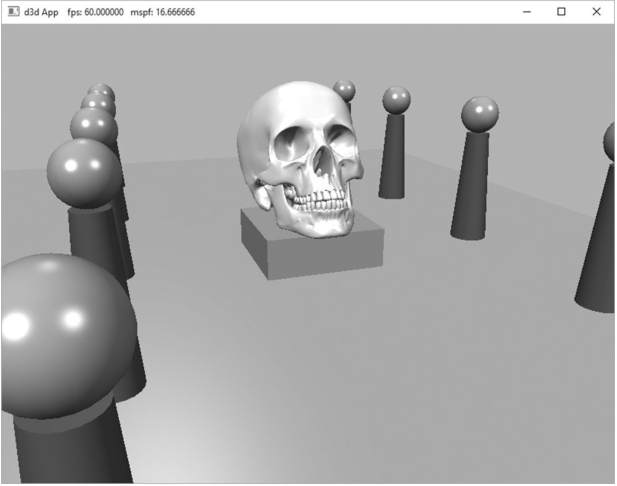
\includegraphics[width=\textwidth]{8-29}
    \centering
    \caption{练习3的截图}
\end{figure}

\begin{flushleft}
4.修改练习3,删除三点光源并在列上方添加以每个球体为中心的点。\\
5.修改练习3,移除三点照明并在列上方添加以每个球体为中心的聚光灯并瞄准。\\
6.卡通风格照明的一个特征是从一种色调到下一种色调的突然过渡(与平滑过渡相反),如图\ref{fig:8-30}所示。 这可以通过以常规方式计算$k_{d}$ 和$k_{s}$来实现,然后在像素着色器中使用它们之前通过离散函数对它们进行转换,如下所示:\\
\end{flushleft}

\begin{align*}
k'_{d}&=f(k_{d})=\left\{\begin{matrix}
0.4 & if & -\infty < k_{d} \leq 0.0 \\ 
0.6 & if & 0.0 < k_{d} \leq 0.5 \\
1.0 & if & 0.5 < k_{d} \leq 1.0 
\end{matrix}\right. \\

k'_{s}&=g(k_{s})=\left\{\begin{matrix}
0.0 & if & 0.0 \leq k_{s} \leq 0.1 \\ 
0.5 & if & 0.1 < k_{s} \leq 0.8 \\
0.8 & if & 0.8 < k_{s} \leq 1.0 
\end{matrix}\right.
\end{align*}

\begin{flushleft}
修改本章的光照演示,使用这种类型的卡通着色。 (注意:上面的函数$f$和$g$只是开始的示例函数,可以调整,直到得到你想要的结果。)
\end{flushleft}

\begin{figure}[h]
    \label{fig:8-30}
    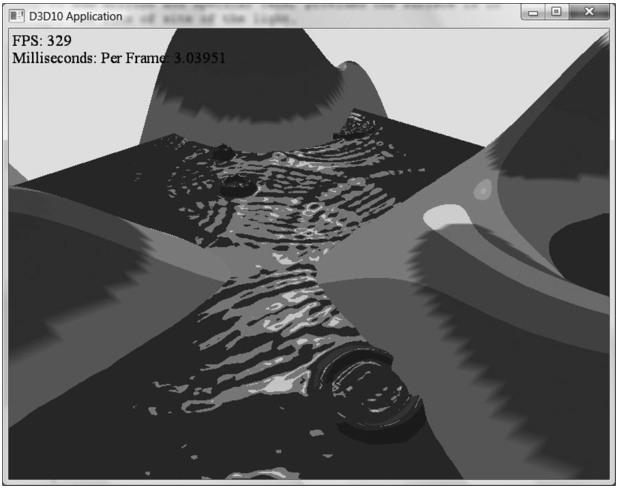
\includegraphics[width=\textwidth]{8-30}
    \centering
    \caption{卡通光照截图}
\end{figure}